\chapter{Grid Computing on Computer Vision}
\label{sec:gridcomputing}
In contemperate computer vision, images are always with high resolution, or video sequences contain long duration and high quality frames. There are massive amount of data in computer vision which are processed in high-dimension, multi-scales, etc. With these massive data, the computational time is enormous. Especially in feature selection, a small number of features are selected from hundreds of thousands features. For instance, Young and Ferryman \cite{Young2005} present that AdaBoost takes a significant amount of time to select Haar features and to learn a good classification. With a 2.8 GHz CPU, the learning for AdaBoost takes about two weeks, and with their optimisation on AdaBoost, the computational time has been improved to 6 hours 47 minutes.

It is clear that the AdaBoost training requires huge amount of computational time, with which there are some difficulties with AdaBoost. First of all, the long duration computational training is very vulnerable to the exceptions of system environment. A standalone long-running program may be corrupted due to memory leak, data loss, processor errors, I/O errors in computer systems. Although these problems are less common in a well designed program, the longer the program is running, the more likely the collapse will occur. For very long duration training, this type of problems is unavoidable. The second difficulty is that there are more computational time required in real-time than expected. In practice, the AdaBoost training is not an ``once a time'' training. It includes many times training with tuning parameters and bias. The actual tuning time is several times larger than the original expected ``once a time'' training time. Grid computing technology is applied to use more computing resources to process the training data simultaneously.

This chapter is organised as follows: \mbox{Section} \ref{sec:introGridComputing}, Grid computing is briefly introduced with its characteristics. In \mbox{Section} \ref{sec:condor}, the general Condor Grid, the Condor Grid at University of Reading and a way to design a computer program for the Condor Grid are introduced. In \mbox{Section} \ref{sec:gridapps}, two computer vision tasks are solved by utilising the Condor Grid. Finally, the advantage and disadvantage of Grid computing are given.

\section{Brief Introduction to Grid Computing}\label{sec:introGridComputing}
The term Grid computing is originated in the early 1990s as a metaphor for making computer power as easy to access as an electric power grid. As a term in distributed computing, Grid computing is explained as several meanings. Some meanings refer to multiple independent computing clusters acting like a ``grid'' because resource nodes are not located within a single domain. Some meanings refer to the creation of a ``virtual supercomputer'' by using spare computing resources within an organisation. And some meanings explain that Grid computing is the creation of a ``virtual supercomputer'' by using a network of geographically dispersed computers.  Among the various meanings, the definition of Grid Computing from \mbox{IBM} is considered as the best one appropriate to the application in this thesis, which says
\begin{quotation}
\textit{A grid is a type of parallel and distributed system that enables the sharing, selection and aggregation of resources distributed across ``multiple'' administrative domains based on their (resources) availability, capacity, performance, cost and users' quality-of-service requirements.}
\end{quotation} 
Grid computing has several characteristics.
\begin{itemize}
 \item Network Centred Parallel Computing
 \item Massive Multiple Computation Power and Data Storage
 \item Lower Cost
 \item CPU Scavenging
\end{itemize}
\paragraph{Network centred parallel computing} 
Grid computing is a type of network centred parallel computing. There is a group of computers which are connected through the network, and processing the parallel tasks. This eases transactions on limited resources as in utility computing, or makes it easier to assemble volunteer computing networks. For example, volunteer computing was popularised in 1999 by the project SETI@home \cite{Anderson2002} which is to solve CPU-intensive research problems, to harness the power of networked personal computers worldwide. One drawback of this feature is that the computers which are involved in performing the computations might not be reliable. The Grid system must be designed to prevent malfunctions or malicious participants from producing false, misleading, or erroneous results. Also, due to the lack of central control, there is no way to guarantee that nodes (computers) will not drop out of the network at random times. Some nodes, like laptops or dialup Internet customers, may also be unavailable for computation when there is no network connection available for unpredictable periods. These drawbacks lead computations fail. In many cases, the participating nodes must be trusty, not to abuse the access that is being granted by the centre system. In this thesis, the grid computation is deployed on a dedicated computer cluster to avoid mistrust and availability difficulties.

\paragraph{Massive multiple computation power and data storage}
Grid computing systems contain massive multiple computation power and data storage. Grids offer a way to solve challenge problems like protein folding, financial modelling, earthquake simulation, and climate/weather modelling. Grids offer a way of using the information technology resources optimally inside an organisation. Some current grid computing systems at least contain hundreds of nodes. Each node is a computer with modern CPU and storage. One of the most famous networks - SETI@home uses more than 3 million computers to achieve $23.37$ sustained teraflops in September 2001. With the massive computation horsepower and huge storage capability, Grid computing is able to tackle some questions which was untouchable technically.

\paragraph{Lower cost (Grid computing v.s. Supercomputers)}
Grid computing costs much less than conventional supercomputers, which includes many processors connected by a high-speed local computer bus. Each node can be purchased as an individual personal computer. When these nodes are connected, they can produce similar computing resources to a multiprocessor supercomputer, but with a lower cost. This is due to the economies of scale of producing personal computers, compared to less economic design and manufacture of customised supercomputers. Conventional supercomputers also cause some physical problems on supplying sufficient electricity energy and cooling capacity in a single location. In Grid computing, the nodes may allocate across several places, and energy consumption for each node is equal to home appliance. The infrastructure and programming considerations on each type of platform are different. It is expensive and difficult to write programs so that they are run in the environment of a supercomputer, because a supercomputer may have a customised operating system, or have some special supported hardware. In Grids, each node has the same infrastructure both on software and hardware due to the standardisation in the IT industry. It is not difficult and not expensive to write programs for common operation systems and hardware.

\paragraph{CPU scavenging}
CPU scavenging is also called \textit{cycle scavenging}, \textit{cycle stealing}, or \textit{shared computing}. CPU scavenging creates a ``grid'' from the unused resources in a network of participants administrative domain. Typically this technique uses computers effectively and prevents computing resources from wasting at night, during lunch, or even in the scattered seconds throughout the day when the computer is waiting for user input or slow devices. The NASA Advanced Supercomputing facility has run genetic algorithms using the Condor cycle scavenger running on about $350$ Sun and SGI workstations. Each workstation runs a daemon that watches user I/O and CPU load. When a workstation has been idle for two hours, a job from the batch queue is assigned to the workstation and will run until the daemon detects a keystroke, mouse motion, or high non-Condor CPU usage. At that point, the job will be removed from the workstation and placed back on the batch queue.

\section{Condor Grid}\label{sec:condor}
Among various Grid computing projects, the Condor grid \cite{Thain2002} is used in this thesis. In this section, the Condor grid is firstly introduced. Then the Condor grid at University of Reading is briefly introduced. The key part is how to design a program for the Condor Grid, which is also given in this section.

\subsection{Condor}
Condor is a research project at the University of Wisconsin-Madison (UW-Madison), and it was first installed as a production system in the UW-Madison Department of Computer Sciences nearly 15 years ago. According to usage statistics on a typical day, Condor delivers more than $650$ CPU days to UW researchers. Today, hundreds of organisations in industry, government, and academia have used Condor to establish compute installations ranging in size from a handful to well over one thousand workstations. Most flavours of Unix are supported, as well as Windows NT/2K and XP.

Condor is a technical workload management system for compute-intensive jobs. Like other batch systems, Condor provides job queueing mechanism, scheduling policy, priority scheme, resource monitoring, and resource management. Users submit their serial or parallel jobs to Condor, Condor places them into a queue, chooses when and where to run the jobs based upon a policy.

\subsection{Condor at UoR}
The Reading University Grid is a Condor Pool consisting of between 200 and 500 nodes. The aim of the Campus Grid is to provide researchers with a High Throughput Computing (HTC) resource. HTC differs from High Performance Computing (HPC) for that it is designed to process tasks that require fairly short processing times (usually minutes or hours), and repeated processes. For example, a program of genetic algorithm takes a sample of data from a data-set, analyses the sample and then stores a result. This process takes 30 minutes but needs to be done $1000$ times. This requires $500$ hours of processing time.

Although nodes in the Condor pool naively run Windows XP,  Cooperative Linux (CoLinux) \cite{Aloni2004} is installed as a Microsoft Windows service on these machines to provide the Linux environment. The CoLinux is an open source software for optimally running Linux on Windows. Specifically, the CoLinux is a port of the Linux kernel that allows it to run together with another operating system on a single machine. For instance, it allows one to freely run Linux on Windows 2000/XP, without using other commercial PC visualisation software such as VMware or Virtual Box. In the University Grid, each node runs on Windows XP, and CoLinux as a diskless Linux image is stored on each node. Once a Windows XP node is idle for a fixed period (such as no I/O access, no keybroad or mouse input), the CoLinux image will be deployed into the memory of nodes. The CoLinux will take over the control of the node. The node becomes running at linux so that it accepts jobs from the Condor pool.

\subsection{Program Design for Condor Grid}
%road-map
The Condor Grid is designed to perform the HTC. It is possible that some HPC is also performed in the Condor Grid. However some modifications are required, and the programs are required to follow some specifications of the Condor Grid. The road-map of running with the Condor Grid is 
%\flushleft
\begin{enumerate}
 \item Preparing code
  \begin{itemize}
      \item separate the whole task into small jobs
     \item define input and output
     \item make the program resume-able
     \item link the program with static-library and compile it
  \end{itemize}
 \item Choosing Runtime Environments (Universe)
\begin{itemize}
 \item standard universe
 \item vanilla universe
\end{itemize}
 \item Generating Submission Description File
\begin{itemize}
 \item executable file
 \item program arguments
 \item input and output data
 \item number of jobs to run
\end{itemize}
 \item Submitting the jobs
 \item Maintaining, Debugging, Adjusting, etc
\end{enumerate}

\subsubsection{Preparing code} An executable program on a stand alone machine can not directly be deployed on the Condor Grid, because the Condor Grid contains a cluster of parallel and distributed individual machines. The original program on a stand alone machine is modified to fit for the specification of the Condor Grid. If the program is designed under an extendable and flexible framework, the modification is minor. However, if the program is designed under a restricted framework, the deployment of whole program is needed to be done. Each machine processes only small part of computation. Therefore, the initial design for the program running on the Condor Grid is to separate the whole task into a large number of small jobs. The number of these jobs should be equal to the number of nodes planned to utilise. Each small job runs on a node.

For any scientific computer program, there must be an input and an output, so when designing a program on the Condor Grid, the input and output of the program must be defined. 

Even if a dedicated grid is allocated, the computation on the grid is not trustworthy. The computation on nodes may fail due to exception of program running, power cuts, system down, and other unpredictable reasons. If computation is broken on a node in a middle way, it has to restart manually from the beginning. It obviously wastes the computational resource. A wise method is to make the program resume-able. A resume-able program uses a log file to record the status of the program at an interval time. If the program is failed in a middle way, it is no need to restart it from the beginning. The program checks the log file, and starts from where it fails.

In compiling the code, the program is linked with static-library. A static library or statically-linked library is a set of routines, external functions and variables which are resolved in a caller at compile-time. The library is copied into a target application by a compiler. Using the static library linking, the program is more independent from different platforms. The compiler produces an object file and a stand-alone executable file. Programs compiled with linking static-libraries normally takes more compiling time and more storage space. 

\subsubsection{Choosing Runtime Environments} The Condor has several runtime environments called universes. There are two universes to choose when submitting a job to the Condor Grid. One is called \textit{standard universe}, and the other is called \textit{vanilla universe}. The standard universe allows a job running under the Condor Grid to handle system calls by returning them to machines where a job is submitted. The standard universe also provides the mechanisms necessary to take a checkpoint and migrate a partially completed job. To use the standard universe, it is necessary to re-link the program with the Condor library and to use the compiler \verb|condor_compile| provided with Condor. The vanilla universe provides a way to run jobs which do not requires to relink. There is no way to take a checkpoint or migrate a job executed under the vanilla universe. For access to input and output files, the jobs must either use a shared file system, or use Condor's File Transfer mechanism. The standard universe provides more flexibilities such as checkpoint and job migration, but it brings some complexity on building the program. The vanilla universe has many constraints on managing the jobs, but the program can be build with any compiler, such as \textbf{GNU GCC} \cite{Gough2004}. In this thesis, the vanilla universe is chosen due to only \textbf{GNU GCC} compiler available.

\subsubsection{Generating Submission Description File} When the runtime environment is decided, jobs are submitted to the Condor pool. The arguments for the submission is described in the submission description file. This file contains commands and keywords to direct the queueing of jobs. In the submission description file, the Condor Grid finds everything it needs to know about the job, such as the name of the executable file, the initial working directory, command-line arguments to the executable file, the directory of input and output data, and the number of jobs to run. It is easy to submit multiple small jobs of a whole task to the Condor pool. The example of the submit description file is below
\begin{verbatim}
Universe = vanilla
Executable = train
Arguments = -job $(Process)
log = log.txt
Error = Error/err.$(Process)
Queue 120 
\end{verbatim} 
This submission description file is to queue $120$ jobs of an executable file \verb|train|. These jobs require the Condor Grid to run the program on machines with different arguments. Each of the $120$ jobs of the program is given its own process arguments, starting with process number $0$. The \verb|$(Process)| represents the current number of process. A log file is assigned to be the file \verb|log.txt|, containing entries about when and where Condor runs, checkpoints, and migrates processes for the $120$ queued jobs. The error message for each job is stored in the file \verb|err.$(Process)| under the directory \verb|Error|. The number of jobs is expressed as \verb|Queue 120|.

\paragraph{Submitting the jobs} Jobs are submitted for execution to the Condor Grid using the \verb|condor_submit| command. 

\paragraph{Maintaining, Debugging, Adjusting, etc.} Once jobs are submitted, the Condor Grid does the rest toward running these jobs, \textit{e.g.}, monitors the jobs' progress with the \verb|condor_q| and \verb|condor_status| commands. The order of these jobs is modified with the \verb|condor_prio| command. The jobs need to be monitored, so that it can find that some jobs stop exceptionally, or some jobs produce wrong output. These jobs need to be stopped and re-submitted manually. This step takes the longest duration in the Condor Grid computation.

\section{Computer Vision Application using Condor Grid}\label{sec:gridapps}
In this section, the Condor Grid has been applied on two computer vision cases which demand large amount of computation. One is to compute mutual information between Gabor wavelet features, the other is to compute the multi-class Gabor-Boosting for feature selection.

\subsection{Computing Mutual Information}
%Mutual information
Refer to Mutual information computation on a whole set of Gabor Feature Pairs (GFPs), the number of GFPs is massive. The purpose of computing mutual information over all GFPs is to find a small group of GFPs which have the lowest mutual information, so that the group of GFPs are formed into a classifier to recognise human faces. There are $30,240$ Gabor features available to construct GFPs. To calculate the mutual information on these $457,213,680$ GFPs, it is necessary to use the Condor Grid utilising the power of hundreds machines.

Among these pairs, they are independent to each other, which means the mutual information on one pair does not affect the mutual information on another pair. Therefore, the whole set of pairs are computed in a parallel way. The whole set of pairs are separated into 121 subsets. Each subset is equivalent to a condor job - roughly $3,700,000$ pairs. If there are enough unclaimed nodes available, $121$ jobs can run simultaneously. The input data for these jobs is the face images from the \mbox{XM2VTS} face database. The output data is stored as a text file recording the quantity of mutual information of each pair for each job. The $121$ jobs are assigned to $121$ nodes in the Condor Grid. \mbox{Figure} \ref{fig:mutCondor} shows the diagram of the Mutual Information Computing with Condor Grid. Through the network, each node takes the input data extracted from the \mbox{XM2VTS} face Database on a machine called \verb|kalypso.rdg.ac.uk|, and stores the output data on a machine called \verb|jupiter.rdg.ac.uk|.
\begin{figure}[ht]
 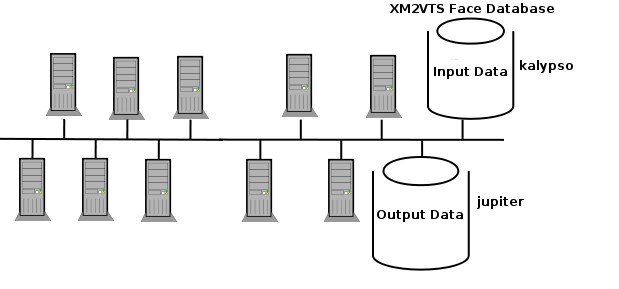
\includegraphics[width=\columnwidth]{ch5/figures/mutCondor.png}
\caption{Computing Mutual Information in the Condor Grid}
\label{fig:mutCondor}
\end{figure} 

If only one stand alone machine is used to calculate the whole set of pairs, it will take a very long duration. For instance, using an \textit{Intel Pentium 4} 2.8 GHz computer, the calculation on each pair takes $20$ milliseconds. The whole set of pairs contains $457,213,680$ GFPs, so that 
\begin{eqnarray}
20\textrm{ millisecond} \times 457213680 \approx 9144273 \textrm{ seconds} \nonumber\\ 
\approx 152404\textrm{ minutes} \approx 2540\textrm{ hours} \approx 105\textrm{ days} \nonumber
\end{eqnarray}
The whole computation will take $105$ days to complete, however it is the optimistic estimation, because the program may failed, be stopped or broken due to some exception happened in the $105$ days.

It is assumed that every node has the same computational capability equal to the \textit{Intel Pentium 4} 2.8 GHz machine on the Condor Gird. Theoretically, the Condor Grid computation on mutual information will take $20$ hours to finish. However, in practice, it takes more time, because the nodes in the Grid are not always dedicated to the Grid computation. Some nodes may be occupied from the Grid computing due to other usages. Also, due to the different hardware configuration on different nodes, the computation capability is different, so that some jobs are finished earlier than others. The whole duration for Condor Grid has been extended for waiting some slow jobs to finish. It indicates that the computational time for the Condor Grid is difficult to predict precisely.

\subsection{Multi-class Gabor-Boosting Feature Selection}
%Multi-class Gabor-Boosting
The second application is to perform the training on Multi-class Gabor-Boosting Feature Selection. The Multi-Class Gabor-Boosting algorithm already has been introduced in \mbox{Section} \ref{tab:multigaborboosting}. The training of mPotsu weak learner is very time consuming, because it includes $200$ individual training on each binary Potsu weak learner respectively. On an \textit{Intel Pentium 4} 2.8 GHz machine, the training on an mPotsu weak learner takes $11$ seconds. It is infeasible to run the training of Multi-class Gabor-Boosting on a stand-alone machine. Therefore, the Condor Grid computation is necessary.

The detailed description of Condor grid implementation is introduced in \mbox{Section} \ref{sec:multifeatureselection} of \mbox{Chapter} \ref{ch:multi}.
%In the Multi-class Gabor-Boosting training, all features are evaluated by building an mPotsu weak learner and calculating the error within each iteration. The evaluation on each feature is independent, because the result from the evaluation of the current feature does not affect the result of the next feature. Hence, the evaluation of each feature can be performed in a parallel way. There are $30,240$ features evaluated in each iteration. The whole set of features are splitted into $120$ subsets, and each subset contains $252$ features. The input data for each job is the face images from the \mbox{XM2VTS} face database. The output data for each job is a text file which records the feature and the error of the corresponding mPotsu weak learner. After all $120$ jobs are finished, an \verb|update| program is to combine all log files into one large file, find the minimum error and the corresponding feature, and update weights for the next iteration. The diagram of the Multi-class Gabor-Boosting training is displayed in \mbox{Figure} \ref{fig:mutliclasscondor}.
%\begin{figure}[ht]
% 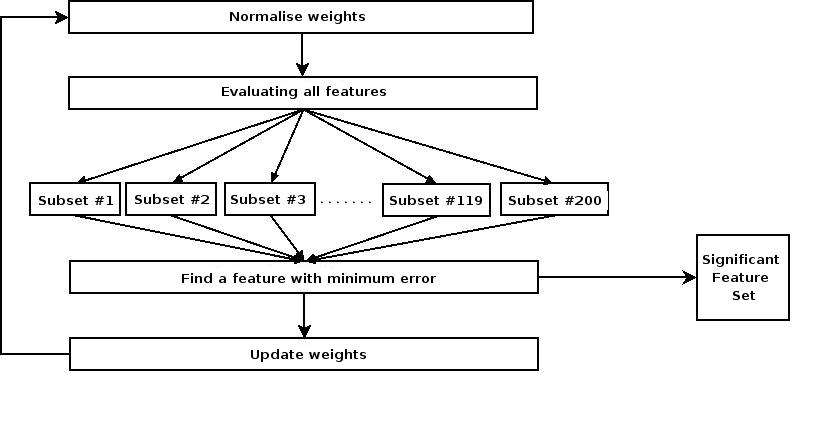
\includegraphics[width=\columnwidth]{ch5/figures/MultiCondor.jpg}
%\caption{The  Multi-class Gabor-Boosting training on the Condor Grid}
%\label{fig:mutliclasscondor}
%\end{figure} 

%If only one \textit{Intel Pentium 4} 2.8 GHz machine is used for the training, each iteration consisting of $30,240$ features will take $332,640$ seconds ($30240\times 11$ seconds), \textit{i.e.}, $92.4$ hours. To select $200$ features from the Multi-class Gabor-Boosting training, the $200$ iterations will take $770$ days, \textit{i.e.}, roughly two year and one month. It is assumed that on the Condor Gird, every node has the same computational capability equal to the \textit{Intel Pentium 4} 2.8 GHz machine. Theoretically, each iteration will take $46.2$ minutes. To select $200$ features, $200$ iterations will be finished in $9,240$ minutes ($46.2\times 200$), \textit{i.e.}, less than one week. Actually, the Condor Grid computation takes more time, but comparing to two years computation, the Condor Grid still displays its advantage over the conventional computation.

\section{Summary}
Grid computing speeds up computer vision application significantly, especially in feature selection. With the Condor Grid, the total computational time is reduced into approximately $1/n$ of the original time ($n$ is the number of nodes) theoretically. In the first computer vision application - mutual information over GFPs, the total computation time has been reduced to $20$ hours instead of $105$ days. In the second computer vision application - Multi-class Gabor-Boosting training, the total computation time becomes less than one week rather than two years. The Grid computing is less expensive comparing to the conventional supercomputers. The Condor Grid consists of a cluster of desktop computers, network connecting nodes, and a sever managing the jobs. The implementation of the Condor Grid is not as difficult as the conventional supercomputers.

However, Grid computing has some shortcomings. For Grid computing, the algorithm must have independent elements so that these elements can be processed in a parallel way. In feature selection, each feature is an element which is independent to each other, so that features are processed in a parallel way. %If an algorithm is not in a parallel way, the algorithm is very difficult to implement with the Grid computing. For instance, the data is needed to fit with the corresponding model by Neural network. The fitting contains millions iterations of neural network computation. The output of the current iteration is the input for the next iteration. Each data example only has a few fixed number of features. The algorithm is not in a parallel way, but in a sequential way. Therefore, the Grid computing is not suitable for this type of computational problem. In addition, the program is required to be well suited to the application. 
The program running in the Condor Grid needs to be processed a small set of data with the cooresponding arguments. Grid computing is not entirely trustworthy. There might be some miss links which lead failure to access input data. In the Condor Grid, the cluster of nodes are not dedicated only for the Grid computing, so that some machines probably are not available after jobs are assigned to them. In this situation, the jobs have to be removed from the Condor Grid, and resubmit to the Condor pool. The performance of the Grid computing is unpredictable, due to different software and hardware configurations on different nodes. It is very hard to predict the computational time of Grid computing. In the Condor Grid computation, the computational time on each node should be kept as small as possible, because when the computational time becomes longer, the more opportunities for the jobs encounter exceptions in running.

In general, Grid computing largely improves computational performance for scientific research. Although it has some drawbacks, these drawbacks can be overcome. Grid computing brings a lot of advantages on computer vision applications.